\documentclass[11pt]{report}

% French packages
\usepackage[utf8]{inputenc}
\usepackage[T1]{fontenc}
\usepackage[francais]{babel}

% Geometry
\usepackage[top=2cm, bottom=2cm, left=3cm, right=3cm]{geometry}

% Fonts
\usepackage{lmodern}

% Outline text
\usepackage{fancybox}

% Custom colors
\usepackage{xcolor}
    \definecolor{lightgray}{rgb}{.9,.9,.9}
    \definecolor{darkgray}{rgb}{.4,.4,.4}
    \definecolor{purple}{rgb}{0.65, 0.12, 0.82}

% Assets path
\usepackage{graphicx}
    \graphicspath{{./assets/}}

\usepackage{lipsum}

% Maths
\usepackage{amsmath}

\usepackage{tikz}
\usetikzlibrary{shapes,snakes}


\usepackage{multicol}

% Display code
\usepackage{listings}
    \definecolor{dkgreen}{rgb}{0,0.6,0}
    \definecolor{gray}{rgb}{0.5,0.5,0.5}
    \definecolor{mallow}{rgb}{0.58,0,0.82}

    % Captions style
    \renewcommand{\lstlistingname}{Source}

    % Listing list style
    \renewcommand\lstlistlistingname{Fichiers source}

    % Custom syntax highlighting
    \lstdefinelanguage{JavaScript}{
      keywords={typeof, new, true, false, catch, function, return, null, catch, switch, var, if, in, while, do, else, case, break class, let, const},
      ndkeywords={class, export, boolean, throw, implements, import, this},
      basicstyle=\ttfamily\scriptsize,
      sensitive=false,
      comment=[l]{//},
      morecomment=[s]{/*}{*/},
      morestring=[b]',
      morestring=[b]""
    }

    \lstset{
        language=JavaScript,
        aboveskip=3mm,
        belowskip=3mm,
        showstringspaces=false,
        columns=flexible,
        basicstyle={\small\ttfamily},
        numbers=none,
        numberstyle=\tiny\color{gray},
        keywordstyle=\color{blue},
        commentstyle=\color{dkgreen},
        stringstyle=\color{mallow},
        breaklines=true,
        breakatwhitespace=true,
        tabsize=4,
        frame=single
    }

% Header/footer
\usepackage{fancyhdr}
    \fancypagestyle{utt}{
        \setlength{\headheight}{23.96pt}
        \fancyfoot[C]{\thepage}
        \fancyhead[L]{\leftmark{}}
        \fancyhead[R]{
\includegraphics[scale=1.5]{logo_utt.jpg}}

        % Rename table of contents
        \addto\captionsfrench{\renewcommand{\contentsname}{Sommaire}}
    }

    \pagestyle{utt}

\title{Rapport - Travail d'investigation Technologique et Scientifique}
\author{Axel \bsc{Mousset} Aurélien \bsc{Labate} \\ Université de Technologie de Troyes}
\date{Printemps 2015}


\begin{document}
    \maketitle
    \chapter*{Remerciements}
    \pagenumbering{gobble}
    \noindent
    Merci à Alexandre Vial pour avoir bien voulu nous encadrer et croire en notre projet.\\
    Merci à Olivier Didon pour avoir réalisé les cartes électroniques du robot.\\
    Merci à Benoit Panicaud pour ses conseils en asservissement.\\
    Merci au club Robotik, pour son cadre de travail et son matériel.\\
    Merci au Bureau des étudiants, à l'institut des sports mécaniques et à l'administration pour leurs subventions.\\
    Et enfin merci à François [nom de famille] pour son usinage irréprochable de la mécanique.\\

    \pagenumbering{arabic}
    \tableofcontents

    \chapter{Introduction}
    L’objectif d’une TITS est de réaliser un projet avec un aspect scientifique de recherche, et
    une mise en application technique en découlant. La robotique, en tant que discipline hybride
    réunit parfaitement ces deux aspects tout en découpant sa dimension technique en un large
    spectre de compétences différentes : électroniques, informatiques et mécaniques, sans parler
    de management et de gestion de projet.\\

    Nous avons donc choisis de mener à bien le développement d’un robot. Les objectifs à
    remplir pour ce robot étaient sa parfaite autonomie, sa capaciter à pouvoir se repérer et se
    déplacer, et la gestion d’une pince mono-axe.
    Ce projet s’inscrit dans une dynamique associative : le robot réalisé a participé à la coupe de
    France de robotique, qui est un concours scientifique à l’échelle nationale réunissant plus de
    200 équipes, sur lequel nous avons finit 54èmes. Ce projet a donc impliqué plus de quatres
    autres personnes régulièrement, étudiants, professeurs, et techniciens de l’UTT. Il est donc
    important de noter que ce document décrit l’essentiel de notre travail, à savoir électronique
    et informatique, mais aussi le projet dans sa globalité car il nous parait pertinent de replacer
    les réalisations dans leurs contexte.
    \chapter{Odometrie}
    L’odometrie désigne l’évaluation de la position du robot dans un repère fixe à l’aide de
    mesures sur son déplacement. On se place dans le cas d’une odométrie calculée à l’aide de deux codeurs incrémentaux à quadrature montés sur roue codeuses. On distingue roues motrices et roues codeuses : en effet, disposer les codeurs directement sur l’arbre moteur risque de provoquer des enregistrement de déplacements liés à un patinage des moteurs en cas de roue motrice bloquée. Les methodes d’odometrie liés à l’utilisation de capteurs optiques ne seront pas traités ici.

    \section{contexte}
        On échantillonne les impulsions des encodeurs périodiquement tous les $d\tau$ . On choisit l’origine au millieu de l’essieu du robot, et on assimile le robot à ce point. La position du robot est représentée par le vecteur
        \begin{equation}
            p = \begin{pmatrix}
                x\\
                y\\
                \theta
            \end{pmatrix}
        \end{equation}

        Avec:
        \begin{itemize}
            \item $(x, y)$ La position du millieu de l’essieu
            \item $\theta$ L'orientation du robot
        \end{itemize}

    \newpage
    \section{Interprétation des signaux}
        \subsection{Valeur et sens de rotation}
        \begin{figure}[h]
            \begin{center}
                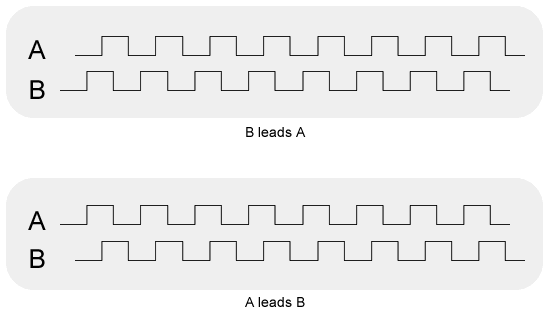
\includegraphics[scale=0.5]{encoder.png}
            \end{center}

            \caption{Signaux envoyés par un encodeur optique rotatif à quadrature}
        \end{figure}
        Chaque encodeur donne deux signaux : le signal A et le signal B. Chaque signal est déphasé de $\pi/4$, et le sens d’un signal peut être déduit de la valeur du deuxième signal au même moment.

        \textbf{Exemple} : l’écoute d’un front montant sur A peut être interpété comme une impulsion positive si l’état de B est à bas au même moment.\\
        On note :
        $$
            \begin{cases}
                impulsions_{gauche}\\
                impulsions_{droite}
            \end{cases}
        $$
        la \textit{somme algébrique des impulsions} depuis le dernier échantillonnage sur les roues gauche et droite.

        \subsubsection{Multiplication logicielle de la résolution}
            Il est possible de multiplier la résolution de son encodeur pour peu qu’il soit de bonne qualité, i.e que le rapport cyclique des signaux envoyés soit de 0.5. Notons que cette multipli-
            cation est purement logicielle, et que par conséquent elle induit une imprécision (bien qu’elle amène aussi une précision suplémentaire du au nombre d’impulsions plus important !).\\
            On peut ainsi doubler la résolution en comptant aussi bien les fronts montant que déscendant sur A, voir même quadrupler si on applique le même principe sur B.\\
            Dans le reste de ce document, on notera $C_r$ le coefficient de résolution, qui représente le nombre de fronts comptés par période du signal.

    \newpage
    \section{Formules de passage}
        On raisonnera la plupart du temps en impulsions d’encodeur et non en mètres. Voyons alors comment passer d’un système à un autre.\\
        On note :
        \begin{itemize}
            \item $impulsions_{parTour}$ le nombre d’impulsion d’encodeur par tour de roue codeuse.
            \item $impulsions_{codeur}$ le nombre d’impulsion d’un tour d’encodeur originel.
            \item $rapport_{reduction}$ le rapport de réduction entre le nombre de tour de roue codeuse et le nombre de tours d’encodeur.\\
        \end{itemize}

        On a la relation suivante :
        \begin{equation}
            impulsions_{parTour} = C_r \times rapport_{reduction} \times impulsion_{encodeur}
        \end{equation}
        Ainsi, pour passer de mètres en impulsions :
        \begin{equation}
            [m] = \frac{[impulsions] \times 2\pi \times R}{impulsions_{parTour}}
        \end{equation}

        \subsubsection{En pratique}
            On utilise le fait que la relation ci-dessus ne fait intervenir que des constantes.\\
            On peut donc la simplifier :
            \begin{equation}
                [m] = K_1 * [impulsions]
            \end{equation}
            Avec $K_1$ le facteur permettant de passer d’un système à l’autre. On le détermine alors empiriquement en faisant parcourir une distance $L$ en mètres au robot et on mesure la distance $\rho$ en impulsions parcourue. On trouve alors :
            \begin{equation}
                K_1 = \frac{L}{\rho}
            \end{equation}

    \newpage
    \section{Traitement des données}
        \begin{figure}[h]
            \begin{center}
                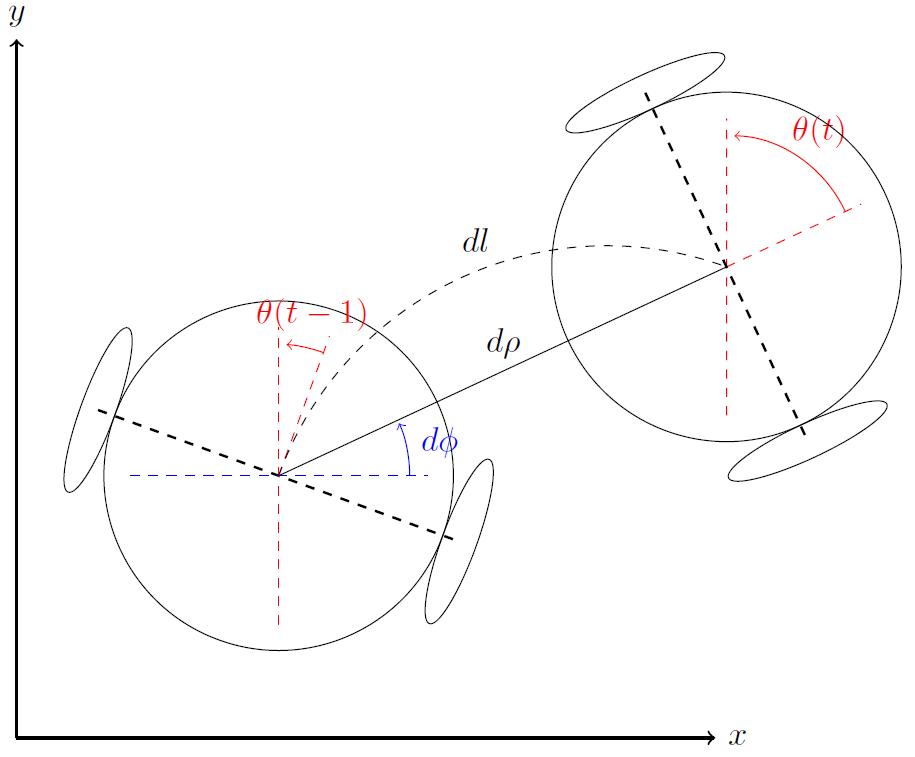
\includegraphics[scale=0.35]{odometry.png}
            \end{center}

            \caption{Evolution du système pendant $d\tau$}
        \end{figure}
        On fait une \textbf{approximation linéaire} sur le déplacement du robot, c’est à dire que l’on considère que sur un intervalle de temps $d\tau$ \textit{assez court} (en pratique 5ms semble suffisant), le déplacement dl du robot est une droite, i.e $d\rho$ = dl.\\
        De même, on consièdre que l’orientation de cette droite est la moyenne de l’orientation en début de déplacement et de l’orientation en fin de déplacement. On note alors $\phi$ l’angle de $d\rho$ :
        $$
            \phi = \frac{\theta(t) + \theta(t-1)}{2} = \theta(t-1)+ \frac{d\theta}{2}
        $$
        Au cours de $d\tau$ à l’instant t :
        \begin{equation}
            d\tau = \frac{impulsions_{gauche} + impulsions_{droite}}{2}
            \label{dTAU}
        \end{equation}
        \begin{equation}
            d\theta = \frac{impulsions_{gauche} - impulsions_{droite}}{entraxe}
            \label{dTHETA}
        \end{equation}
        Avec entraxe la distance entre le centre des deux roues codeuses.\\

        \textbf{En pratique} : Comme pour le facteur de passage entre ticks et mètres, la valeur de l’entraxe utilisée sur le système final doit être déterminée \textbf{empiriquement}. On fait alors tourner le robot sur $n\pi$ en sommant la différence de ticks. On trouve alors :
        \begin{equation}
            entraxe = \frac{\sum(impulsions_{gauche} - impulsions_{droite})}{n\pi}
        \end{equation}

        \newpage
        On procède à une intégration numérique\footnote{i.e une somme discrète, considérée continue car $d\tau$ est petit} pour obtenir l’orientation du robot dans le repère fixe:
        $$
            \theta(n) = \int_0^t d\theta
        $$
        Pour obtenir les coordonnées du robot dans le repère fixe, on projette la droite portée par $\rho$.
        \begin{equation}
            dx = d\rho \times cos(\theta(t-1) + \frac{d\theta}{2})
        \end{equation}
        \begin{equation}
            dy= d\tau \times sin(\theta(t-1) + \frac{d\theta}{2})
        \end{equation}
        A nouveaupar intégration numérique, on obtient les coordonnées du robot dans le repère fixe:
        $$ x(t) = \int_0^t dx $$
        $$ y(t) = \int_0^t dy $$
        Finalement, en notant $p$ la position du robot, on peut éxprimer $p'$ sa position après un échantillonnage.
        \begin{equation}
            p' =
            \begin{pmatrix}
                x\\
                y\\
                \theta
            \end{pmatrix} +
            \begin{pmatrix}
                \frac{impulsions_{gauche}+impoulsions_{droite}}{2}\times cos(\theta+\frac{impulsions_{gauche}-impulsions_{droite}}{2\times entraxe})\\
                \frac{impulsions_{gauche}+impoulsions_{droite}}{2}\times sin(\theta+\frac{impulsions_{gauche}-impulsions_{droite}}{2\times entraxe})\\
                \frac{impulsions_{gauche}-impulsions_{droite}}{entraxe}
            \end{pmatrix}
        \end{equation}

        \newpage
        \subsubsection{Code d'exemple}
            \begin{lstlisting}[language=JavaScript]
// Constantes theoriques
const REFRESH_TIME = 5; //ms
const RESOLUTION_COEF = 2;
const ENCODER_TICKS = 500;
const REDUCTOR_RATIO = 1.2;
const WHEEL_RADIUS = 0.06; //metres
const ENTRAXE = metersToTicks(0.5); //impulsions

let leftEncoder = new Encoder();
let rightEncoder = new Encoder();
let distance = 0;
let orientation = 0;
let x = 0;
let y = 0;
let lastCall = null;

function ticksToMeters(ticks) {
    return (ticks * 2 * Math.PI * WHEEL_RADIUS) /
        (RESOLUTION_COEF *REDUCTOR_RATIO * ENCODER_TICKS);
}

function metersToTicks(meters) {
    return (meters * RESOLUTION_COEF *REDUCTOR_RATIO * ENCODER_TICKS) /
        (2 * Math.PI * WHEEL_RADIUS);
}

/**
* Fonction de rafraichissement appelee le plus frequemment possible
*/
function compute() {
    let now = Date.now();
    // On s’assure que les calculs sont fait a intervalles reguliers
    if (now - previousOrientation >= REFRESH_TIME) {
        lastCall = now;
        let leftTicks = leftEncoder.getTicks();
        let rightTicks = leftEncoder.getTicks();
        leftEncoder.resetTicks();
        rightEncoder.resetTicks();
        let rho = (leftTicks + rightTicks) / 2;
        let dTheta = (leftTicks - rightTicks) / ENTRAXE;
        let dx = rho * Math.cos(orientation + dTheta / 2);
        let dy = rho * Math.sin(orientation + dTheta / 2);
        x += dx;
        y += dy;
        orientation += dTheta;
    }
}

function getRobotStatus() {
    return {
        x : ticksToMeters(x),
        y : ticksToMeters(y),
        orientation: orientation
    }
}
        \end{lstlisting}
    \chapter{Asservissement}
    Que ce soit en robotique ou dans différents processus industriels, il est souvent indispensable de contrôler certaines grandeurs physiques.
    On appelle \textbf{asservissement} d'une grandeur l'ensemble des moyens permettant de contrôler \textbf{automatiquement} cette grandeur.\\
    Celui-ci peut être mis en place soit au moyen d'un \textit{système en boucle ouverte}, c'est a dire en calculant une commande sans prendre en compte la réponse du système: le système nécessite alors une parfaite modélisation, nous ne nous attarderons donc pas sur ce type d'asservissement.\\
    L'asservissement dont nous allons parler se place dans le cas d'un \textbf{système en boucle fermée} ou \textbf{système à contre réaction négative}, qui, contrairement à son homologue ouvert, mesure la réaction du système pour adapter la commande. Toute la difficulté est alors de réussir à déterminer la fonction permettant d'adapter la commande de sortie en fonction de l'objectif voulu et du résultat mesurée.\\
    Le correcteur \textit{PID} est un exemple de système à boucle fermée permettant d'asservir efficacement une grandeur. C'est le correcteur le plus utlisié, qui a largement fait ses preuves dans l'industrie.
    \begin{figure}[h]
        \centering
        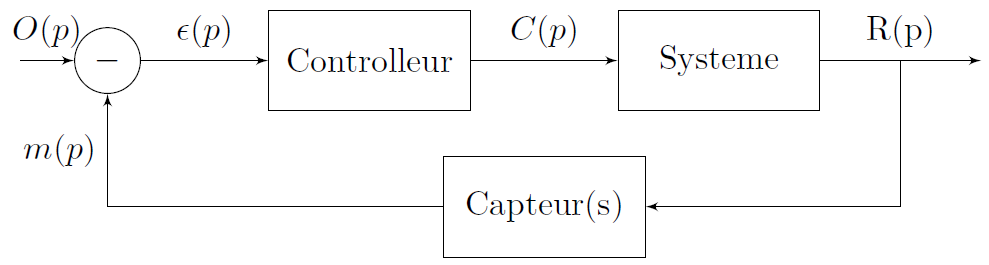
\includegraphics[scale=0.35]{assets/ASSERV.png}
        \caption{Représentation d'un système asservi en boucle fermée}
    \end{figure}


    \newpage
    \section{Correcteur PID}
        Le correcteur PID est un système à contre réaction \textbf{négative}, il calcule donc une commande en fonction de l'erreur $\epsilon$ de la grandeur, c'est à dire la différence entre la valeur voulue (i.e l'objectif) $O$, et valeur mesurée $m$.
        \begin{equation}
            \epsilon (t) = O(t) - m(t)
        \end{equation}
        La commande de sortie, passée au travers d'un correcteur PID, qu'on note $C(t)$, consiste en une somme de trois termes: une réponse proportionnelle à l'erreur, une réponse proportionnelle à la somme des erreurs, et une réponse proportionnelle à l'évolution de l'erreur. Une traduction quasi-litéralle de cette définition nous donne la relation suivante:
        \begin{equation}
            C(t) = f(\epsilon(t)) = K_p . \epsilon(t) + K_i . \int_{0}^{t}\epsilon(\tau).d\tau + K_d . \frac{d\epsilon}{dt}(t)
        \end{equation}
        Ou plus simplement\footnote{Les relations mettant en jeux des intégrales et des dérivées sont plus simples à exprimer dans le domaine de Laplace} dans le domaine de Laplace:
        \begin{equation}
            C(p) = f(\epsilon(p)) = K_p . \epsilon(p) + K_i . \frac{\epsilon(p)}{p} + K_d.p.\epsilon(p)
        \end{equation}
        Ce que l'on peut résumer à l'aide du schéma-bloc suivant:
        \begin{figure}[h]
            \centering
            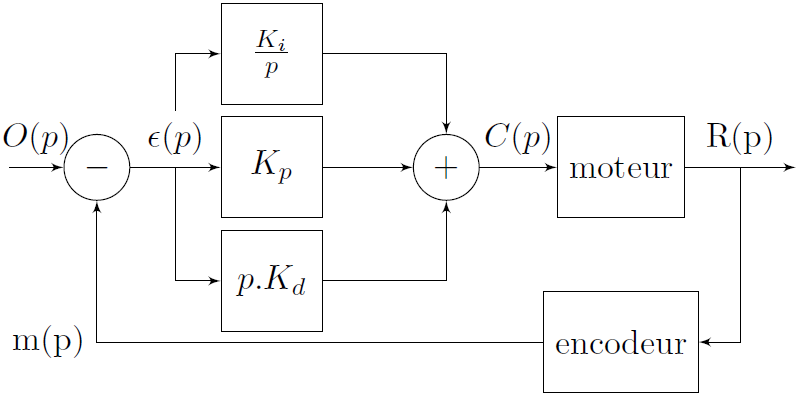
\includegraphics[scale=0.35]{assets/PID.png}
            \caption{Représentation d'un correcteur PID}
        \end{figure}

        \newpage
        \subsection{Influence des coefficients}
            Dans cette section, allons présenter l'influence des différents coefficients sur le système. En guise d'introduction à chacun d'eux, nous allons faire le parallèle avec un système (une voiture) et son correcteur pouvant être assimilé à un PID (un conducteur). On se place dans le cas ou sur une route, le conducteur décide d'être éxactement à la limite de la distance de sécurité de la voiture d'en face.

            \subsubsection{Réponse proportionnelle}
                \textit{«Plus je suis loin de la limite, plus je dois appuyer sur la pédale d'accélération.»}\\
                Le terme proportionnel permet de répondre aux grandes inerties du système, et diminue le temps de montée en donnant l'essentiel de la puissance au moteur: plus l'erreur est grande, plus la réponse est importante. La valeur de $K_p$ est proportionnelle à la vitesse de réaction du système. L'erreur statique est réduite avec l'augmentation de $K_p$, cependant le système perd en stabilité. En cas de $K_p$ démesuré, le système oscille et ne trouve jamais stabilité.\\
                Dans le cas d'un moteur, une variation trop faible de tension ne fait plus varier sa vitesse. Ainsi lorsque l'erreur devient trop faible, le terme proportionel ne permet pas de combler une erreur statique qui est d'autant plus faible que $K_p$ est grand.

            \subsubsection{Réponse intégrale}
                \textit{«Moins j'accélère pour une pression de la pédale d'accélération donnée, plus je dois appuyer sur la pédale.»}\\
                Le terme intégral fait la somme algébrique des erreurs. Il permet ainsi de donner une réponse de plus en plus forte à mesure que le système persiste dans son erreur. Il complète ainsi le terme proportionel, car permet de combler l'erreur statique laissée par ce dernier en régime permanent.\\
                Augementer $K_i$ permet de diminuer l'impact de faibles perturbations, augemente la précision du système en régime permanent. Un $K_i$ trop important peut cependant augementer le dépassement de la consigne «overshoot», et causer d'oscillations semblables à celles du $K_p$ en cas de valeur démesurée.

            \subsubsection{Réponse dérivée}
                \textit{«Plus j'accélère vite et que je me rapporoche de la limite (et risque donc de la dépasser), moins je dois appuyer sur la pédale.»}\\
                L'action du terme dérivé dépend du signe et de la vitesse de variation de l'erreur. Sa valeur va donc s'opposer à la réponse proportionnelle et intégrale. Elle devient importante lorsque l'erreur faiblit grandement et que le terme proportionnel continue à donner de grandes valeurs: elle freine le système empéchant le dépassement de la consigne et diminuant les petites oscillations qui ralentissent la stabilisation du système. $K_d$ compense donc $K_p$ lorsque l'erreur faiblit, on peut ainsi pousser $K_p$ pour limiter l'erreur statique quitte à dépasser la consigne, puis compenser ce dépassement en augementant $K_d$.

        \newpage

        \subsection{Réglage des coefficients}
            Régler les coefficients représente la majeure difficulté de la mise en place d'un asservissement PID. On s'intéresse ici uniquement à l'asservissement d'un moteur (à courant continu, ou pas).

            \subsubsection{Méthode théorique: Modélisation du système}
            Dans un premier temps, il est toujours intéressant de s'intéresser à la réponse théorique du système. Cette méthode n'est donc pas une méthode complète en soit, mais juste un outil permettant de "dégrossir" les coefficients avant de les affiner sur le système final.\\
            Les démonstrations des fonctions de transfert ci-dessous ne seront pas développées ici, car elle ne font pas l'objet de ce document. En effet, seul le modèle final et son utilisation nous intéresse.\\
            La fonction de transfert entre la vitesse angulaire de sortie et la tension d'entrée d'un moteur peut être modélisée comme un filtre du second ordre:
            \begin{equation}
                H(p) = \frac{\omega(p)}{U(p)} = \frac{A}{1 + \frac{2.\xi}{\omega_0} + \frac{1}{\omega_0^2}.p^2}
            \end{equation}
            Avec:
            \begin{itemize}
                \item $\omega(p)$ Vitesse de rotation du rotor
                \item $U(p)$ Tension appliquée au moteur
                \item $A = \frac{1}{K_e}$ Gain statique
                \item $\omega_0 = \sqrt{\frac{K_e.K_c}{L.J_T}}$ Pulsation propre
                \item $K_e/K_c$ Constante de vitesse/couple
                \item $J_T$ Moment d'inertie apporté au rotor
            \end{itemize}

            \paragraph{Moteur à courant continu}{
                \begin{itemize}
                    \item $\xi = \frac{R}{2}\sqrt{\frac{J_T}{K_e.K_c.L}}$ Facteur d'amortissement
                    \item $R$ Résistance au bornes du moteur
                    \item $L$ Inductance du moteur
                \end{itemize}
            }


            \paragraph{Moteur sans balais}{
                \begin{itemize}
                    \item $\xi = \frac{3R}{2}\sqrt{\frac{J_T}{K_e.K_c.L}}$ Facteur d'amortissement
                    \item $Ke = 0,0605.K_t$
                    \item $R$ Résistance phase-à-phase
                    \item $L$ Inductance phase-à-phase\\
                \end{itemize}
            }
            Il est possible de modéliser le moment d'inertie $J_T$ perçu par le moteur sur son arbre dans le cas d'une utilisation sur un robot de masse $M$ en connaissant le rayon des roues $R$.
            \begin{equation}
                J_T = M.R^2
            \end{equation}

            \newpage
            \subsubsection{Méthode empirique 1: dite de «Ziegler-Nichols»}
                La méthode de Ziegler-Nichols ne nécessite aucune modélisation au préalable, seule une batterie d'éssais expérimentaux souvent automatisables est nécessaire.\\
                Le principe est de fixer $K_i$ et $K_d$ à 0, puis d'augementer $K_p$ jusqu'à obtenir une réponse oscillante en régime permanent. On mesure alors la période $T_osc$ de cette réponse à $(K_p)_{lim}$.\\
                Les coefficients sont déduits de ces deux mesures par les relations suivantes:
                \begin{equation}
                \begin{cases}
                    K_p = 0.6 . (K_p)_{lim}\\
                    K_i = \frac{1}{0.5 . T}\\
                    K_d = 0.125 . T
                \end{cases}
                \end{equation}
                Les coefficients déduits sont assez polyvalents car ils proposent un bon compromis entre rapidité, dépassement de la consigne, stabilité, et précision. Néammoins, selon la spécification de la réponse désirée, il est possible d'ajuster les différents coefficients à la main. Par exemple, dans le cas de l'asservissement d'un robot, on va vouloir limiter au maximum le dépassement de consigne et donc baisser $K_p$.

            \subsubsection{Méthode empirique 2: dite «À la main»}
                Cette dernière méthode est utile lorsque l'on a des besoins spécifiques quant à la réponse du système. Par exemple, sur un asservissement en position, on peut vouloir complètement éliminer le dépassement de la consigne (il peut être critique d'aller trop loin et de déplacer un objet à la coupe de France !), quitte à avoir un temps de stabilisation plus long. Dans ce cas là, un asservissement de type PD est recommendable. Le principe est de faire varier $K_p$ jusqu'à qu'il y ai dépassement de consigne, puis de compenser en augmentant $K_d$ jusqu'à élimination de l'erreur statique.

    \section{Asservissement en vitesse}
        Première manière de contrôler le déplacement du robot: on asservit indépendemment chaque moteur en vitesse.\\
        Incovénient: pour aller à une position donnée, il faut donc intégrer numériquement les consignes de vitesse.
    \subsubsection{Code d'exemple}
            \begin{lstlisting}[language=JavaScript]
function velocityControl() {
    let velocity = encoder.getTicks(); // Vitesse en implusion par DeltaT
    encoder.resetTicks();

    previousVelocityError = velocityError;
    velocityError = velocityObjective - velocity;

    let derivative = velocityError - previousVelocityError; // On inclut le 1/DeltaT dans K_d
    integral += velocityError;

    velocityCommand = kp * velocityError + ki * integral + kd * derivative;

    return velocityCommand;
}
            \end{lstlisting}

    \newpage
    \section{Asservissement en position}
        Asservir indépendemment chaque moteur en position permet de résoudre le  problème d'intégration numérique. Par contre, la vitesse n'étant plus asservie, l'accélération peut être beaucoup trop grande, on s'expose alors à des risques de dérapages.
    \subsubsection{Code d'exemple}
            \begin{lstlisting}[language=JavaScript]
function positionControl() {
    position += encoder.getTicks(); // Position en ticks
    encoder.resetTicks();

    previousPositionError = positionError;
    positionError = velocityObjective - velocity;

    let derivative = positionError - previousPositionError; // On inclut le 1/DeltaT dans pKd
    integral += positionError;

    positionCommand = pKp * positionError + pKi * integral + pKd * derivative;

    return positionCommand;
}
            \end{lstlisting}

    \section{Asservissement en vitesse et en position}
        Réunir à la fois un asservissement en vitesse et en position permet de réunir le meilleur des deux mondes. On peut controller la vitesse, et donc l'accélération tout en se passant d'intégration numérique grace à l'asservissement en position.\\
        Un premier asservissement en position va donner une consigne de vitesse, qui après traitement algorithmique pour écrêter vitesse et accélération, va servir de consigne pour un deuxième asservissement en vitesse. On est donc capable de faire atteindre aux moteurs n'importe quelle position tout en controlant la vitesse ainsi que l'accélération à laquelle ils y vont.

        \subsubsection{Choix du profil de vitesse}
        Le profil de vitesse adopté est trapézoïdal. On commence par une phase d'accélération jusqu'à une vitesse de croisière, puis une déccélération jusqu'à atteindre la position voulue. L'avantage est de ne pas brusquer les moteurs, de ne pas déraper au démarrage et de ne pas dépasser l'objectif de position par inertie.

        \begin{figure}[h]
            \centering
            
\begin{tikzpicture}
% horizontal axis
\draw [->] (0,0) -- (8cm,0) node[below] {$t$};

% vertical axis
\draw[->] (0,0) -- (0,4cm) node[anchor=east] {$V$};

\foreach \x in {0,1,2,3,4, 5, 6, 7}
    \draw (\x cm,1pt) -- (\x cm,-1pt) node[anchor=north] {};
\foreach \y in {0,1,2,3}
    \draw (1pt,\y cm) -- (-1pt,\y cm) node[anchor=east] {};

% nominal speed
\draw[dotted] (2,0) -- (2,4);
\draw[dotted] (5,0) -- (5,4);

% Us
\draw[thick] (0,0) -- (2,2) -- (5,2) -- (7,0);
\draw (0.7,1.5) node {$A_{max}$}; %label
\draw (3.5,2.5) node {$V{max}$}; %label
\draw (6.3,1.5) node {$-A_{max}$}; 

\end{tikzpicture}
            \caption{Profil de vitesse trapézoïdal}
        \end{figure}

        \newpage

        Au niveau de l'algorithme, on tronque juste la valeur de la vitesse si elle dépasse une valeur $V_{max}$. On fait de même avec l'accélération en tronquant sa valeur absolue à $A_{max}$.
        \subsubsection{Code d'exemple}
            \begin{lstlisting}[language=JavaScript]
function motionControl() {
    previousVelocityObjective = positionCommand;
    velocityObjective = positionControl();

    // Ecretage de la vitesse
    if (Math.abs(velocityObjective) > maxVelocity) {
        velocityObjective = sign(velocityObjective) * maxVelocity;
    }

    let acceleration = velocityObjective - previousVelocityObjective;
    // Ecretage de l'acceleration
    if (Math.abs(acceleration) > maxAcceleration) {
        velocityObjective = previousVelocityObjective + sign(acceleration) * maxAcceleration;
    }

    motor.run(velocityControl());
}
            \end{lstlisting}

    \newpage
    \section{Asservissement polaire}
        Jusqu'à présent, tous les types d'asservissement proposés se faisaient sur une ou deux grandeurs, indépendemment sur chaque moteur. Il est possible de travailler sur des grandeurs «couplée», réunissant les informations fournies par les deux moteurs.\\

        Pour un robot, il peut être intéressant d'asservir sur la position et l'orientation. L'intérêt est de pouvoir facilement envoyer le robot à une une position $(x, y, \theta)$, sans avoir à faire du traitement algorithmique pour déterminer les consignes de position à envoyer à chaque moteur comme dans un asservissement position ou position/vitesse.\\
        On a donc en tout quatre controlleurs PID: deux pour un asservissement position/vitesse sur la vitesse de déplacement du robot, et deux pour un asservissement position/vitesse sur la vitesse angulaire du robot.\\
        Les grandeurs mesurées ne sont plus directement les impulsions d'encodeur, mais les variations de vitesse et de vitesse angulaire calculées par l'odométrie et décrites par les relations \eqref{dTAU} et \eqref{dTHETA} pour les PID de vitesse, et l'orientation/distance globale pour les PID de distance.

        \subsubsection{Code d'exemple}
            \begin{lstlisting}[language=JavaScript]
function robotControl() {
    /*
        Quadruple asservissement position/vitesse sur la distance et l'angle
        calcules par l'odometrie
    */
    let distanceVelocityCommand = distanceMotionControl();
    let orientationVelocityCommand = orientationMotionControl();

    /*
        Signe arbitraire. On part du principe que l'angle est calcule avec la
        difference entre la position gauche et droite
     */
    leftMotor.run(distanceVelocityCommand - orientationVelocityCommand);
    rightMotor.run(distanceVelocityCommand + orientationVelocityCommand);
}
            \end{lstlisting}

    \chapter{Conclusion}
    La réalisation du robot a été menée à son terme dans les délais que nous nous étions imposé pour concourrir à la coupe de France. Néanmoins, une casse de nature mécanique a empêché le robot d'être oppérationnel dès le premier jour. Ainsi, le robot secondaire (développé par d'autres étudiants) a quand même pu marquer des points.\\

    Malgré cet accident, ce projet nous a donné satisfaction. C'est en effet un réel projet d'ingénierie, alliant autant compétences scientifiques, techniques et humaines pendant plus de six mois d'efforts motivés par l'envie de performer dans une compétition.\\

    Au niveau personnel, l'ensemble des connaissances acquises est très enrichissant. Il a fallu effectuer un large travail documentaire en amont sur des sujets comme l'automatisation, l'asservissement ou encore l'odométrie. C'est donc avec passion que nous nous sommes attachés à mettre en pratique ces nouvelles connaissances aux côtés de celles apprises en cours pour réaliser ce robot.\\

    A un niveau plus large, nous éspérons que ce travail pourra répondre à l'une des problématique majeure dans le monde associatif à l'UTT, à savoir la transmission des savoirs. Le projet a donc largement été penser pour devenir potentiellement de base de référence pour futures années du club de robotique de l'UTT.

    \appendix
    \include{chapters/06-Annexes}

    \nocite{*}
    \bibliographystyle{plain-fr}
    \bibliography{references}
\end{document}